\documentclass[a4paper, 12pt, oneside]{book}
\usepackage[italian]{babel}
\usepackage[T1]{fontenc}
\usepackage[utf8]{inputenc}
\usepackage{graphicx} 
\usepackage{hyperref}
\usepackage{float}
\usepackage{listings}
\usepackage[dvipsnames]{xcolor}
\usepackage[
    type={CC},
    modifier={by-nc-sa},
    version={4.0},
]{doclicense}

\pagestyle{plain}

\lstset{
    language=Java,
    basicstyle=\ttfamily\small,
    keywordstyle=\color{blue}\bfseries,
    commentstyle=\color{Green},
    stringstyle=\color{purple},
    numbers=none,
    numberstyle=\tiny\color{gray},
    stepnumber=1,
    tabsize=3,
    frame=tb,
    aboveskip=3mm,
    belowskip=3mm,
    columns=flexible,
    breaklines=true,
    breakatwhitespace=true,
    showstringspaces=false
}

\title{Sviluppo di un'applicazione software per la pianificazione personalizzata di un calendario di gare di trail running}
\author{Ivan Gaudino}
\date{A.A. 2023/2024}

\begin{document}
\begin{titlepage}
    \centering
    
\includegraphics[width=0.8\textwidth]{images/polito_logo_2021_blu}
    \begin{center}
        \LARGE\textbf{Politecnico di Torino}
    \end{center}
    \begin{center}
        \Large{Corso di Laurea Triennale in Ingegneria Gestionale}\\
        \Large{Classe L-8: Ingegneria dell'Informazione}\\
        \Large{A.A. 2023/2024}
    \end{center}
    \vspace{10pt}
    \begin{center}
        \LARGE\textbf{Sviluppo di un'applicazione software per la pianificazione personalizzata di un calendario di gare di trail running}
    \end{center}
    \vspace{4cm}
    \begin{flushleft}
        \large\textbf{Relatore \hfill Candidato}\\
        \large{Prof. Giuseppe Bruno Averta \hfill Ivan Gaudino}
    \end{flushleft}
\end{titlepage}

\newpage
\thispagestyle{empty}
\mbox{}
\frontmatter
\tableofcontents
\listoffigures

\mainmatter
\chapter{Proposta di progetto} \label{cap:proposta}
\section{Titolo della proposta}
Sviluppo di un'applicazione software per la pianificazione personalizzata di un calendario di gare di trail running.

\section{Descrizione del problema proposto}
Ogni anno si svolgono gare di trail running (corsa su sentieri in ambiente naturale) in molti paesi del mondo e la maggior parte di esse, soprattutto quelle più conosciute, richiede l'iscrizione con parecchi mesi di anticipo, poiché il numero di partecipanti è spesso limitato. Oltre che iscriversi, gli atleti che intendono partecipare ad una gara vogliono anche arrivarci preparati fisicamente e mentalmente per ottenere il miglior risultato possibile. Questo richiede una preparazione, con allenamenti costanti, che l'atleta vuole programmare con un margine di tempo sufficiente.

Si vuole offrire all'atleta un'applicazione in grado di pianificare le gare a cui vuole/può partecipare, sulla base di filtri e preferenze indicate dall'atleta stesso.

\section{Descrizione della rilevanza gestionale del problema}
Per un atleta appassionato di trail running che vuole partecipare a più gare durante l'anno, può essere certamente utile sfruttare un'applicazione che permetta di creare una programmazione personalizzata delle gare, basata su filtri e preferenze selezionati dall'atleta stesso. In questo modo, l'atleta può iscriversi alle gare di interesse con congruo anticipo, senza il rischio di trovare chiuse le iscrizioni a causa del raggiungimento del numero massimo di partecipanti, e può inoltre pianificare con cura gli allenamenti, la dieta e tutto quello che ritiene necessario per arrivare preparato alla gara, riducendo la probabilità di infortuni o scarsi risultati.

\section{Descrizione dei data-set per la valutazione} \label{sec:descrizione-dataset}
Il dataset utilizzato è reperibile sulla piattaforma Kaggle, con il titolo \href{https://www.kaggle.com/datasets/mgpoirot/utmb-world-race-daa}{\textit{UTMB world race data}}\footnote{\color{blue}\url{https://www.kaggle.com/datasets/mgpoirot/utmb-world-race-daa}}.

La tabella include dettagli e risultati di più di 38.000 gare di trail running svolte dal 2014 al 2024. Non tutte le colonne saranno rilevanti al fine del funzionamento dell'applicazione; di seguito vengono riportati i campi di interesse con relativa descrizione:
\begin{enumerate}
    \item Race UID (INT): codice univoco della gara
    \item Year (INT): anno
    \item Day (INT) : giorno, numero intero a partire dal 1 Gennaio
    \item Race Title (VARCHAR): nome della gara
    \item N Participants (INT): numero di partecipanti
    \item Race Category (VARCHAR): categoria della gara (20K, 50K, 100K, 100M)
    \item Distance (FLOAT): lunghezza della gara, in km
    \item Elevation Gain (INT): dislivello positivo della gara
    \item Mean Finish Time (DOUBLE): tempo medio in ore dei partecipanti che hanno concluso la gara
    \item Winning Time (DOUBLE): tempo in ore del vincitore
    \item Last Time (DOUBLE): tempo in ore dell'ultimo classificato
    \item N DNF (INT): numero di partecipanti ritirati dalla gara
    \item N Women (INT): numero di partecipanti donne
    \item Raw Location (VARCHAR): città/paese in cui si svolge la gara
    \item Continent (VARCHAR): sigla del continente
    \item Country (VARCHAR): sigla della nazione
\end{enumerate} 

\section[Descrizione preliminare degli algoritmi coinvolti]{Descrizione preliminare degli algoritmi \\ coinvolti} \label{sec:algoritmi-coinvolti}
L'applicazione prevede il calcolo di una lista di gare, tra quelle presenti nel dataset, mediante un algoritmo ricorsivo che lavora sulla base dei filtri inseriti dall'utente. Ogni filtro mira a rendere la soluzione finale la più appropriata possibile alle preferenze dell'utente, nonché a ridurre la complessità computazionale dell'algoritmo date le dimensioni del dataset. Quest'ultima regola non si applica per il filtro \textit{livello di abilità}: l'utente può scegliere tra \textit{principiante}, \textit{intermedio} o \textit{esperto}, e la scelta va a definire alcuni vincoli sulle categorie di gare che l'atleta può correre e sul numero minimo di giorni che deve intercorrere tra una gara e la successiva, a seconda della loro categoria. Questo insieme di vincoli contribuisce a generare soluzioni quanto più ottimali e realistiche, ma aumenta il carico computazionale perché richiede numerosi controlli e calcoli durante l'esecuzione dell'algoritmo.

Ad esser meno realistico è il filtro \textit{anno}, con il quale si vuole far selezionare all'utente l'anno a cui vuole fare riferimento per la pianificazione delle gare. Il motivo della presenza di questo filtro è legato soprattutto alla costruzione del dataset: non tutte le gare si svolgono ogni anno e per una stessa gara (stesso \textit{Race UID}), al variare dell'anno, vi sono più campi discordanti quali il giorno, il numero di partecipanti, i risultati e il nome stesso, che nel dataset spesso include anche l'anno di riferimento o comunque differisce di anno in anno, per cui risulterebbe inappropriato raggruppare le gare secondo il loro codice univoco \textit{Race UID}.

L'obiettivo dell'algoritmo ricorsivo viene scelto dall'utente: 
\begin{itemize}
    \item \textbf{Massimizzare il numero di gare}: la soluzione conterrà il maggior numero possibile di gare
    \item \textbf{Massimizzare i km da percorrere}: la somma dei km delle gare appartenenti alla soluzione sarà la più elevata possibile
    \item \textbf{Massimizzare il numero di nazioni in cui svolgere le gare}: la soluzione includerà il maggior numero possibile di nazioni in cui si svolgono le gare
\end{itemize}
A seconda dell'obiettivo scelto, l'algoritmo proporrà all'utente una soluzione ottimale costituita da una lista di gare riportante, per ognuna, la data, il luogo, il nome, i chilometri da percorrere e il dislivello.

\section{Descrizione preliminare delle funzionalità previste per l’applicazione software}
La scheda principale dell'applicazione permette di definire i criteri per il calcolo della pianificazione personalizzata delle gare. A tale scopo, l'utente specifica le proprie preferenze mediante i seguenti filtri:
\begin{itemize}
    \item \textbf{Livello di abilità}: \textit{principiante}, \textit{intermedio}, o \textit{esperto}. Come descritto nella sezione \ref{sec:algoritmi-coinvolti}, la scelta del livello impone alcuni vincoli predefiniti per rendere il problema e le soluzioni il più realistiche possibile
    \item \textbf{Anno}: l'anno di riferimento per il calcolo della soluzione, dal 2014 al 2024
    \item \textbf{Continenti}: la soluzione includerà gare che si svolgono nei continenti selezionati
    \item \textbf{Nazioni}: la soluzione includerà gare che si svolgono nelle nazioni selezionate
    \item \textbf{Mesi da escludere}: le gare che si svolgono nei mesi selezionati saranno escluse dalla soluzione
    \item \textbf{Categoria preferita}: \textit{20K}, \textit{50K}, \textit{100K} e \textit{100M}. La soluzione sarà composta per almeno il 50\% da gare della categoria scelta
    \item \textbf{Gara preferita}: le gare visualizzate saranno compatibili con i filtri selezionati. La gara scelta sarà sicuramente inclusa nella soluzione
    \item \textbf{Numero massimo di gare}: la soluzione sarà formata al massimo dal numero di gare indicato
    \item \textbf{Km massimi per gara}: le gare facenti parte della soluzione non supereranno questo limite
\end{itemize}
L'applicazione prevede anche la presenza di una seconda scheda, denominata \textit{Scopri il tuo livello}. Qui l'utente può inserire i dettagli delle gare già disputate e i risultati ottenuti, e lasciare che sia l'applicazione a determinare il livello di abilità. Per farlo, l'applicazione farà riferimento ai dati \textit{Mean Finish Time}, \textit{Winning Time} e \textit{Last Time} presenti nel dataset per quelle gare.

Dalla scheda principale, l'utente può scegliere l'obiettivo per il calcolo della pianificazione delle gare tra le seguenti opzioni: massimizzare il numero di gare a cui partecipare, massimizzare i chilometri da percorrere o massimizzare il numero di nazioni in cui svolgere le gare. L'applicazione mostrerà la soluzione come elenco di gare con relativi dettagli.

\chapter{Descrizione del problema affrontato}
\section{Contesto operativo}
Il \textbf{trail running} è un'attività fisica all'aperto che prevede la corsa su sentieri naturali. A differenza della corsa su strada o su pista, il trail running si svolge su terreni variabili e irregolari, come terreni di montagna, collina e sterrati, caratterizzati da dislivelli sia positivi che negativi. Il percorso segue le pendenze naturali del suolo e la natura gioca quindi un ruolo fondamentale: andatura, attrezzatura, stile e tecnica di corsa devono adattarsi al sentiero. 

Nel 2015 il trail running è stato riconosciuto come una disciplina dell'atletica leggera e negli ultimi anni è diventato sempre più popolare; secondo la \textit{International Track and Field Federation} il trail running è uno degli sport in più rapida crescita al mondo. I paesaggi particolarmente suggestivi, il senso di avventura, la varietà dei percorsi, il rispetto per la natura, così come anche l'accessibilità e la ridotta competitività rispetto alla corsa su strada, sono alcuni dei fattori che hanno contribuito alla crescente popolarità del trail running. Inoltre, diversi marchi di abbigliamento e attrezzatura sportiva stanno investendo molto in questa disciplina, sponsorizzando eventi, gare e atleti, nonché creando intere collezioni di prodotti specializzati. 

\section{Rilevanza del problema scelto}
Le gare di trail running si suddividono in quattro categorie: \textit{20K} per le brevi distanze, \textit{50K} per le distanze medie tra i 50 e i 100 km, \textit{100K} per le lunghe distanze intorno ai 100 km, e \textit{100M} per le ultramaratone di oltre 170 km. Le quattro categorie di gara si basano sul coefficiente di \textit{chilometro-sforzo}, una formula riconosciuta a livello mondiale per misurare la distanza di gara nel trail running, che considera sia la distanza che il dislivello per calcolare la distanza percepita\footnote{\color{blue}\url{https://utmb.world/it/sports-system}}. Distanza percorsa e dislivello, insieme a tipo di terreno, condizioni atmosferiche e altri fattori, rendono ogni gara un'esperienza unica che richiede un'attenta preparazione fisica e mentale. Per questo, la pianificazione delle gare può essere molto importante per un atleta, sia amatoriale che professionista, per vari motivi:
\begin{itemize}
    \item \textbf{Iscrizione alle gare}: molte gare, soprattutto quelle più conosciute, hanno posti limitati e richiedono l'iscrizione con diversi mesi di anticipo 
    \item \textbf{Allenamenti e dieta}: un giusto piano di preparazione fisica, mentale e alimentare può migliorare le prestazioni in gara
    \item \textbf{Risultati}: se si vuole competere per i primi posti in classifica, è bene poter definire degli obiettivi per mantenere risultati costanti
    \item \textbf{Recupero fisico}: i periodi di recupero sono fondamentali. Una corretta pianificazione della frequenza delle gare aiuta a prevenire infortuni e sovraccarichi fisici 
    \item \textbf{Mobilità}: si può voler partecipare a gare all'estero o lontane da casa, quindi sarà necessario organizzare i viaggi e il pernottamento
\end{itemize}

\section{Potenzialità e criticità}
L'applicazione sviluppata si propone come uno strumento che, considerati i punti sopra elencati, offra all'atleta, o all'utente in generale, una pianificazione personalizzata di un calendario di gare di trail running per facilitarlo nella gestione del suo percorso sportivo. L'algoritmo ricorsivo agisce in questo senso e cerca di trovare una soluzione ottimale tenendo conto delle preferenze dell'utente e dei vincoli più importanti, come la frequenza delle gare, la loro compatibilità con il livello di abilità dell'atleta e la gestione dei tempi di recupero fisico. Inoltre, la possibilità per l'utente di scegliere l'obiettivo della pianificazione secondo le opzioni elencate alla fine della sezione \ref{sec:algoritmi-coinvolti} rende l'applicazione ancora più flessibile.

L'algoritmo potrebbe tenere conto anche di modalità di accesso particolari per alcune gare, come sorteggi o qualifiche, che si applicano specialmente agli eventi più famosi. Tuttavia, questo richiederebbe un dataset molto specifico e dettagliato e una gestione più complessa dell'applicazione.

\chapter{Descrizione del data-set utilizzato per l'analisi}
Il dataset utilizzato per l'analisi è costituito da tre tabelle: \textbf{races}, \textbf{continents} e \textbf{countries}. La prima, descritta nella sezione \ref{sec:descrizione-dataset}, è quella principale e include dettagli e risultati di più di 38.000 gare di trail running svolte dal 2014 al 2024. Alcune righe della tabella presentavano campi vuoti per le colonne \textit{Mean Finish Time}, \textit{Winning Time} e \textit{Last Time}; queste righe sono state rimosse perché avrebbero potuto causare eccezioni nell'applicazione nella scheda \textit{Scopri il tuo livello}, durante il calcolo automatico del livello di abilità dell'utente.

La tabella \textit{races} contiene informazioni geografiche (\textit{Continent} e \textit{Country}) sottoforma di codice ISO 3166-1 alpha-2. Per visualizzare questi dati in modo comprensibile, sono state utilizzate le tabelle \textit{continents} e \textit{countries}. Esse sono composte da due colonne ciascuna e riportano il codice ISO 3166-1 alpha-2 e il nome esteso, la prima per i sette continenti e la seconda per le nazioni del mondo. Entrambe le tabelle sono state create manualmente.

\begin{figure}[t]
    \vspace*{-7cm}
    \centering
    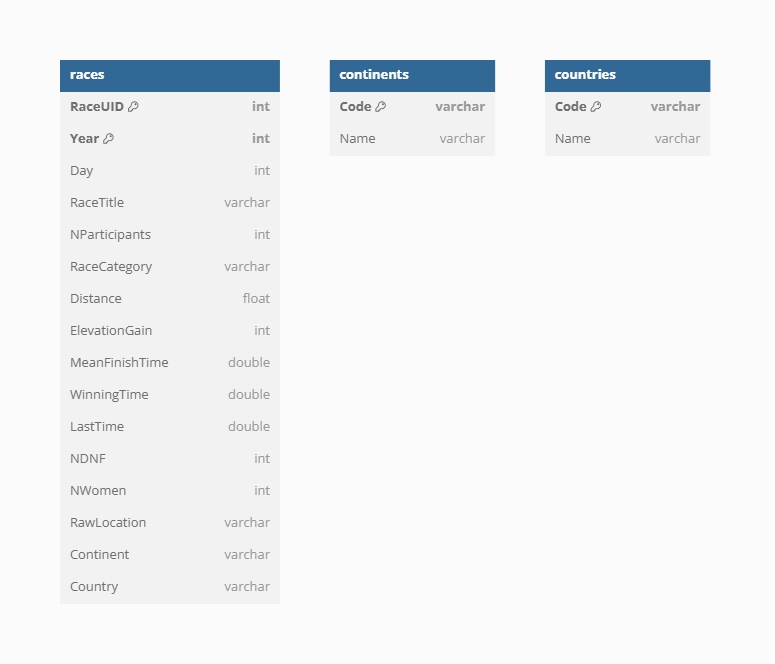
\includegraphics[width=\textwidth]{images/dataset_tables.png}
    \caption{Tabelle dataset}
    \label{fig:tabelle-dataset}
\end{figure}

\chapter{Strutture dati e algoritmi utilizzati}
\section{Struttura del progetto}
L'applicazione è stata sviluppata in linguaggio Java, seguendo i pattern di programmazione MVC (\textit{Model-View-Controller}), per mantenere separata la logica dell'applicazione dall'interfaccia utente, e DAO (\textit{Data Access Object}), per isolare la logica di accesso ai dati. Adottando questo approccio, il progetto viene suddiviso in tre pacchetti:
\begin{itemize}
    \item \textbf{RacePlanner}: contiene le classi per l'avvio e l'inizializzazione dell'applicazione, e i \textit{controller} per la gestione delle interazioni dell'utente con l'interfaccia
    \item \textbf{RacePlanner.db}: comprende le classi per la configurazione dell'accesso al database e l'estrazione dei dati
    \item \textbf{RacePlanner.model}: racchiude la logica algoritmica e applicativa, e le classi che modellano gli oggetti
\end{itemize}

\begin{figure}[h]
    \centering
    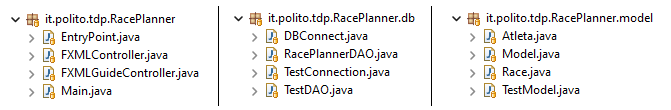
\includegraphics[width=0.8\textwidth]{images/panoramica_packages.png}
    \caption{Panoramica pacchetti}
    \label{fig:packages}
\end{figure}

\section{Logica applicativa}
L'applicazione risponde in modo dinamico alle interazioni dell'utente con l'interfaccia. Questo richiede numerosi controlli e validazioni a livello del Controller e una corretta manipolazione dei dati da parte del Model. Tutti i campi di input dell'interfaccia sono associati a metodi di gestione degli eventi che monitorano delle modifiche sui campi eseguite dall'utente. 

Particolare rilevanza ha il metodo che estrae la lista di gare valide, che quindi rispettano vincoli e filtri impostati dall'utente, utile poi all'algoritmo ricorsivo per calcolare la soluzione. Questa lista è aggiornata dinamicamente, riflettendo le selezioni dell'utente sugli elementi di input. Viene qui riportato il codice del metodo:
\begin{lstlisting}
    void handleCmbAction(ActionEvent event) {
    	cmbFavRace.getItems().clear();
    	lblWarnings.setText("");
    	btnGare.setDisable(false);
		btnKm.setDisable(false);
		btnNazioni.setDisable(false);
    	String lvl = cmbLevel.getValue();
    	Integer anno = cmbYear.getValue(); 
    	List<String> continenti = ckCmbContinents.getCheckModel().getCheckedItems();
    	List<String> nazioni = ckCmbNations.getCheckModel().getCheckedItems();
    	List<String> mesiNo = ckCmbMonths.getCheckModel().getCheckedItems();
    	// le condizioni sulle CheckComboBox risolvono un bug della libreria ControlsFX
    	if(lvl!=null && anno!=null && !continenti.contains("null") 
    			&& !nazioni.contains("null") && !mesiNo.contains("null")) {
    		String favCat = cmbCategory.getValue();
    		try {
    			List<Race> filteredRaces = model.getFilteredRaces(lvl, favCat, anno, continenti, nazioni, mesiNo);
    			cmbFavRace.setDisable(false);
    			this.isFavRaceEmpty = false;
    			Collections.sort(filteredRaces);
    			cmbFavRace.getItems().addAll(filteredRaces);
    		} catch(IllegalArgumentException e) {
    			btnGare.setDisable(true);
    			btnKm.setDisable(true);
    			btnNazioni.setDisable(true);
    			lblWarnings.setText(e.getMessage());
    		} catch(IllegalStateException e) {
    			cmbFavRace.setDisable(true);
    			this.isFavRaceEmpty = true;
    		}
    		
    	} else {
    		cmbFavRace.setDisable(true);
    	}
    }
\end{lstlisting}
Il metodo legge i valori impostati sui filtri e invia le istruzioni al metodo del Model \textit{getFilteredRaces}, che si occupa di:
\begin{itemize}
    \item inviare al DAO i parametri per la costruzione dell'interrogazione al database
    \item costruire la lista di gare valide e popolarla degli oggetti estratti dal dataset
    \item restituire la lista al Controller o generare eccezioni di cui si occuperà il Controller di gestire 
\end{itemize}
Anche l'interrogazione al database è strutturata per essere dinamica, cioè in grado accettare un numero di parametri variabile. A tal fine, viene utilizzata la classe Java \textit{StringBuilder} per la manipolazione delle stringhe, insieme ai controlli sui parametri. Si riporta l'estratto di codice per la costruzione della query:
\begin{lstlisting}
    public List<Race> getRaces(Integer anno, List<String> categorie,
			List<String> continenti, List<String> nazioni) {
		StringBuilder sql = new StringBuilder("SELECT r.*, n.Name FROM races r, continents c, countries n "
				+ "WHERE r.Continent=c.Code AND r.Country=n.Code AND r.Year=? ");
		
		if(categorie!=null && !categorie.isEmpty()) {
			sql.append("AND r.RaceCategory IN (");
			for(int i=0; i<categorie.size(); i++) {
				sql.append("?,");
			}
			sql.deleteCharAt(sql.length() - 1);
			sql.append(") ");
		}
		
		if(continenti!=null && !continenti.isEmpty()) {
			sql.append("AND c.Name IN (");
			for(int i=0; i<continenti.size(); i++) {
				sql.append("?,");
			}
			sql.deleteCharAt(sql.length() - 1);
			sql.append(") ");
		}
		
		if(nazioni!=null && !nazioni.isEmpty()) {
			sql.append("AND n.Name IN (");
			for(int i=0; i<nazioni.size(); i++) {
				sql.append("?,");
			}
			sql.deleteCharAt(sql.length() - 1);
			sql.append(") ");
		}
        ...
    }
\end{lstlisting} 

\section{Algoritmi} \label{sec:algoritmi}
I due principali algoritmi dell'applicazione sono il metodo ricorsivo per il calcolo ottimale della pianificazione e quello per la valutazione del livello di abilità dell'atleta. In termini di complessità computazionale, mentre il secondo algoritmo esegue operazioni aritmetiche sui dati, il primo rappresenta un problema di ottimizzazione combinatoria. 

Per l'implementazione dell'algoritmo ricorsivo, viene costruito un grafo semplice, pesato e orientato, i cui vertici sono l'insieme delle gare valide. Due gare sono collegate da un arco se la prima gara precede cronologicamente la seconda e se tra le due è rispettato il vincolo sul numero minimo di giorni che deve intercorrere tra due gare, data la loro categoria e il livello di abilità dell'atleta. L'arco è orientato nel verso che segue l'ordine cronologico e ha come peso il numero di giorni di distanza tra le due gare. Di seguito viene mostrata la traduzione in codice di queste istruzioni: 
\begin{lstlisting}
    private void creaGrafo(String lvl) {
		this.grafo = new SimpleDirectedWeightedGraph<>(DefaultWeightedEdge.class);
		Graphs.addAllVertices(this.grafo, this.gareValide);
		
		Collections.sort(this.gareValide, new Comparator<Race>() {
			@Override
			public int compare(Race r1, Race r2) {
				return r1.getDate().compareTo(r2.getDate());
			}	
		});
		
		Atleta atleta = this.getAtleta(lvl);
		for(int i=0; i<gareValide.size(); i++) {
			Race r1 = gareValide.get(i);
			LocalDate dateR1= r1.getDate();
			int giorniMin = atleta.getMapCategoriaGiorni().get(r1.getRaceCategory());
			for(int j=i+1; j<gareValide.size(); j++) {
				Race r2 = gareValide.get(j);
				LocalDate dateR2= r2.getDate();
				long giorniTraGare = ChronoUnit.DAYS.between(dateR1, dateR2);
				if(giorniTraGare >= giorniMin && giorniTraGare >= 15) { //la minima distanza in giorni assoluta e' 15
					Graphs.addEdge(grafo, r1, r2, giorniTraGare);
				}
			}
		}
	}
\end{lstlisting}
Il grafo così creato ha uno scopo fondamentale: ridurre il carico computazionale dell'algoritmo e, quindi, migliorarne le prestazioni. Rispetto ad un approccio di ricerca esaustiva con complessità N!, che esplorerebbe tutte le combinazioni, il grafo permette di restringere il campo di ricerca andando a considerare solo le combinazioni valide. Nonostante ciò, considerate le notevoli dimensioni del dataset, il numero di combinazioni rimane significativamente elevato, e questo, insieme ai controlli di validità che vengono chiamati ad ogni passo ricorsivo, aumentando ulteriormente il tempo di esecuzione, rappresentano la maggiore criticità dell'algoritmo. A tal proposito, affinare il più possibile le preferenze sui filtri è essenziale per l'utente, permettendo all'algoritmo di mantenere buone prestazioni e trovare la soluzione ottimale in tempi ragionevoli. 
% Adottare un approccio euristico per la ricerca di una soluzione approssimata potrebbe essere una scelta computazionalmente più efficiente, ma volendo mantenere la ricerca di una soluzione ottimale ...   

L'algoritmo ricorsivo è suddiviso in due metodi: il primo riceve i parametri dal Controller e inizializza gli attributi necessari per la ricorsione, il secondo esegue la ricorsione vera e propria. Quest'ultimo metodo è replicato in tre versioni, una per ciascun obiettivo (massimizzare il numero di gare, i chilometri da percorrere o il numero di nazioni). Ciò che differisce tra le tre versioni sono le condizioni di controllo della soluzione migliore, mentre il passo ricorsivo condivide gli stessi controlli sui vincoli. Di seguito è riportato il codice del metodo ricorsivo per la ricerca della soluzione ottimale che massimizza il numero di gare: 
\begin{lstlisting}
    private void massimizzaGare(String button, String lvl, List<Race> parziale, String favCat, Integer maxGare, Float maxKm) {
		if(maxGare!=null && parziale.size() > maxGare) {
			return;
		}
		
		if(parziale.size() > best.size()) {
			this.best = new ArrayList<>(parziale);
		}
		
		for(DefaultWeightedEdge e : grafo.outgoingEdgesOf(parziale.get(parziale.size()-1))) {
			Race gara = Graphs.getOppositeVertex(grafo, e, parziale.get(parziale.size()-1));
			if(!parziale.contains(gara) && isAggiuntaValida(parziale, gara, maxKm, favCat, lvl)) {
				parziale.add(gara);
				this.incrementaContatori(button, gara, favCat, lvl);
				
				massimizzaGare(button, lvl, parziale, favCat, maxGare, maxKm);
				
				parziale.remove(parziale.size()-1);
				this.decrementaContatori(button, gara, favCat, lvl);
			}
		}
	}
\end{lstlisting}
La ricorsione si avvia con una lista di oggetti \textit{Race}, chiamata \textit{parziale}, che rappresenta una possibile soluzione. Nel metodo di inizializzazione, alla lista \textit{parziale} viene aggiunta una gara come punto di partenza, estratta dal set di vertici del grafo. L'algoritmo esplora tutti i possibili cammini del grafo partendo ogni volta da un vertice diverso, così da coprire tutte le gare come potenziali punti di partenza. 

Per l'esplorazione dei cammini, la ricorsione si concentra sull'ultimo elemento aggiunto a \textit{parziale}. Per ogni gara collegata ad esso con un arco, l'algoritmo verifica se può essere aggiunta a \textit{parziale} controllando che soddisfi i vincoli. In caso positivo, la gara viene aggiunta alla lista e l'algoritmo entra in una nuova chiamata ricorsiva. Se la soluzione rappresentata da \textit{parziale} è migliore della miglior soluzione finora trovata (\textit{best}), allora quest'ultima viene aggiornata con il contenuto di \textit{parziale}. Al termine della chiamata ricorsiva per una gara, l'algoritmo esegue il \textit{backtracking}: rimuove l'ultima gara aggiunta e continua l'esplorazione dei cammini con le altre gare collegate al vertice corrente. Quando la ricorsione termina, \textit{best} rappresenterà la soluzione ottimale trovata.

Per quanto riguarda l'algoritmo di determinazione del livello di abilità dell'atleta, questo si basa su operazioni aritmetiche e confronti tra i dati inseriti dall'utente, passati come parametro dal Controller, e i campi \textit{Mean Finish Time}, \textit{Winning Time} e \textit{Last Time} del dataset, salvati negli oggetti \textit{Race}. Gli input dell'utente vengono ricevuti dal Model tramite una mappa avente come chiave un oggetto \textit{Race} e come valore il tempo ottenuto dall'atleta in quella gara. Segue il codice del metodo: 
\begin{lstlisting}
    public String findLevel(Map<Race, LocalTime> raceTimeMap) {
		List<Integer> listLevel = new ArrayList<>();
		for(Race gara : raceTimeMap.keySet()) {
			double inf = (gara.getMeanFinishTime() + gara.getLastTime()) / 2;
			double sup = (gara.getMeanFinishTime() + gara.getWinningTime()) / 2;
			double tempoDecimale = localTimeToDecimalHours(raceTimeMap.get(gara));
			if(tempoDecimale >= inf)
				listLevel.add(0);
			else if(tempoDecimale < inf && tempoDecimale > sup)
				listLevel.add(1);
			else if(tempoDecimale <= sup)
				listLevel.add(2);
		}
		
		int sum = 0;
		for(Integer lvl : listLevel) {
			sum += lvl;
		}
		
		double media = sum / listLevel.size();
		
		if(media >= 0 && media <= 0.5)
			return "Principiante";
		else if(media > 0.5 && media <= 1.4)
			return "Intermedio";
		else if(media > 1.4 && media <= 2)
			return "Esperto";
		
		return null;
	}
\end{lstlisting}
Il metodo, per ogni gara presente nella mappa ricevuta come parametro, divide l'intervallo \textit{Last Time - Winning Time} in tre sotto-intervalli. In base al sotto-intervallo in cui ricade il tempo ottenuto dall'atleta per quella gara, viene aggiunto un valore (0, 1 o 2) a una lista. Il valore medio degli elementi presenti nella lista stabilirà il livello di abilità dell'atleta.

\chapter{Diagramma delle classi principali}
\begin{figure}[h]
    \centering
    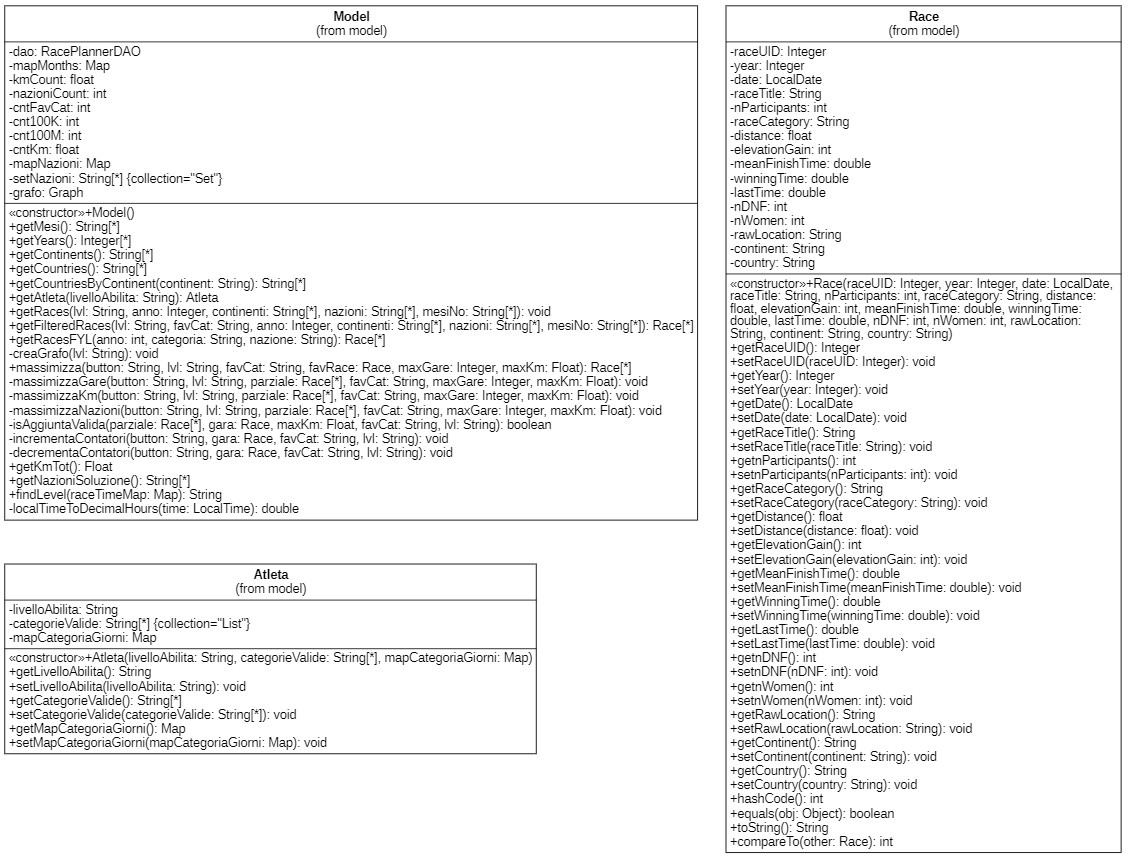
\includegraphics[width=\textwidth]{images/UML_package_model.png}
    \caption{Diagrammi UML delle classi del package model}
    \label{fig:uml-model}
\end{figure}

\begin{figure}[t]
    \vspace{-0.8cm}
    \centering
    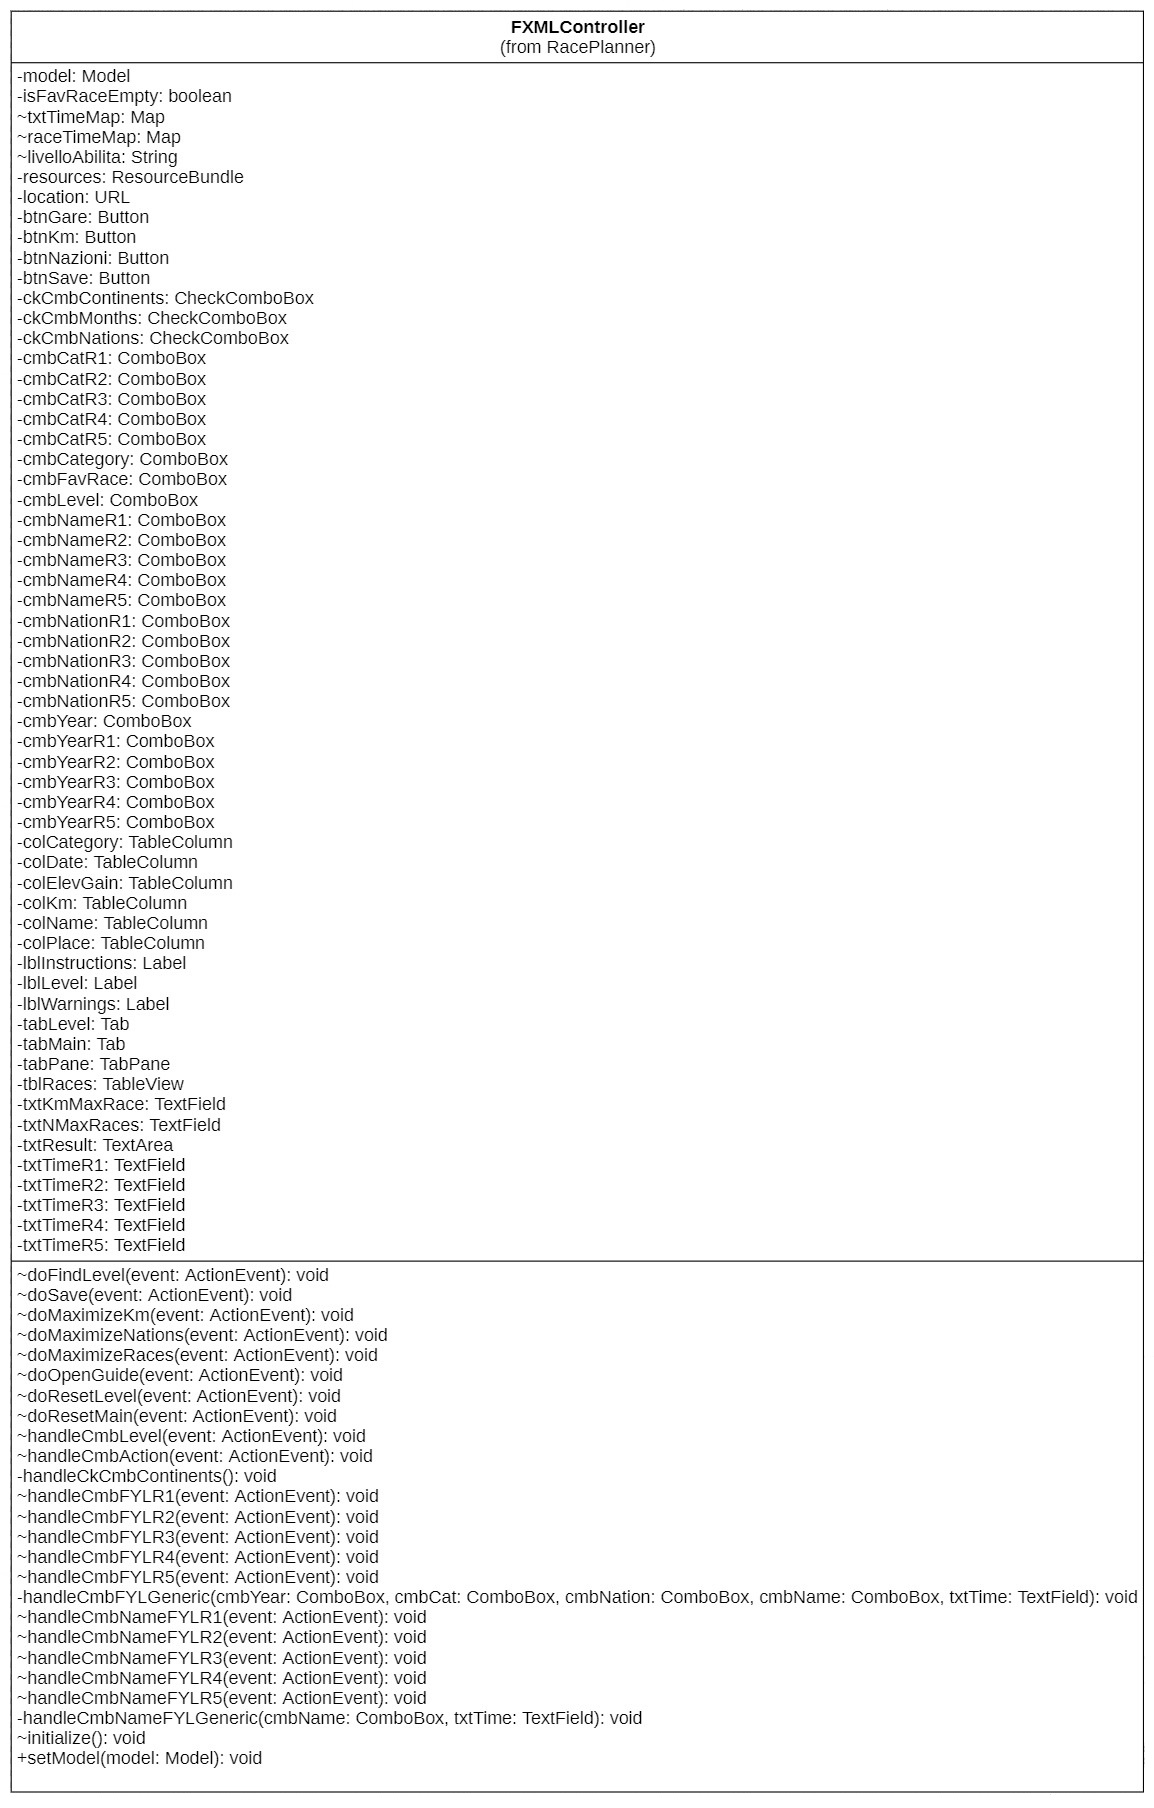
\includegraphics[width=0.65\textwidth]{images/UML_controller.png}
    \caption{Diagramma UML della classe FXMLController}
    \label{fig:uml-controller}
\end{figure}

\begin{figure}
    \centering
    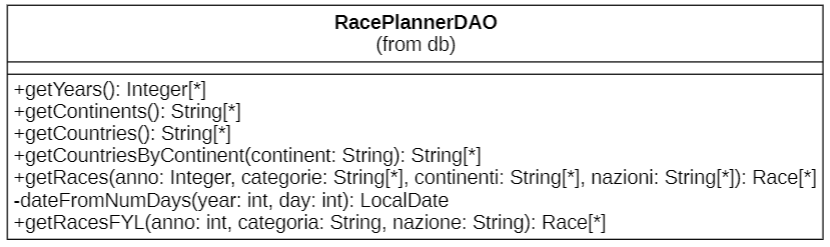
\includegraphics[width=0.7\textwidth]{images/UML_dao.png}
    \caption{Diagramma UML della classe RacePlannerDAO}
    \label{fig:uml-dao}
\end{figure}

\chapter{Interfaccia dell'applicazione} \label{cap:interfaccia}
L'interfaccia grafica è stata realizzata in JavaFX con l'ausilio del software Scene Builder ed è composta da due sezioni: la scheda \textit{Principale} e la scheda \textit{Scopri il tuo livello}.

La scheda \textit{Principale} è dedicata alla pianificazione del calendario di gare. Gli elementi che compongono la scheda sono elementi di input (\textit{ComboBox}, \textit{CheckComboBox} e \textit{TextField}) per la selezione delle preferenze dell'utente, pulsanti, una tabella e un'area di testo per mostrare i risultati. La tabella mostra il calendario con i dettagli di ciascuna gara nella soluzione, mentre l'area di testo fornisce un riepilogo della soluzione, includendo il numero di gare, la somma dei chilometri, e l'elenco delle nazioni in cui si svolgono le gare. 
% figura tab principale vuoto
\begin{figure}
    \centering
    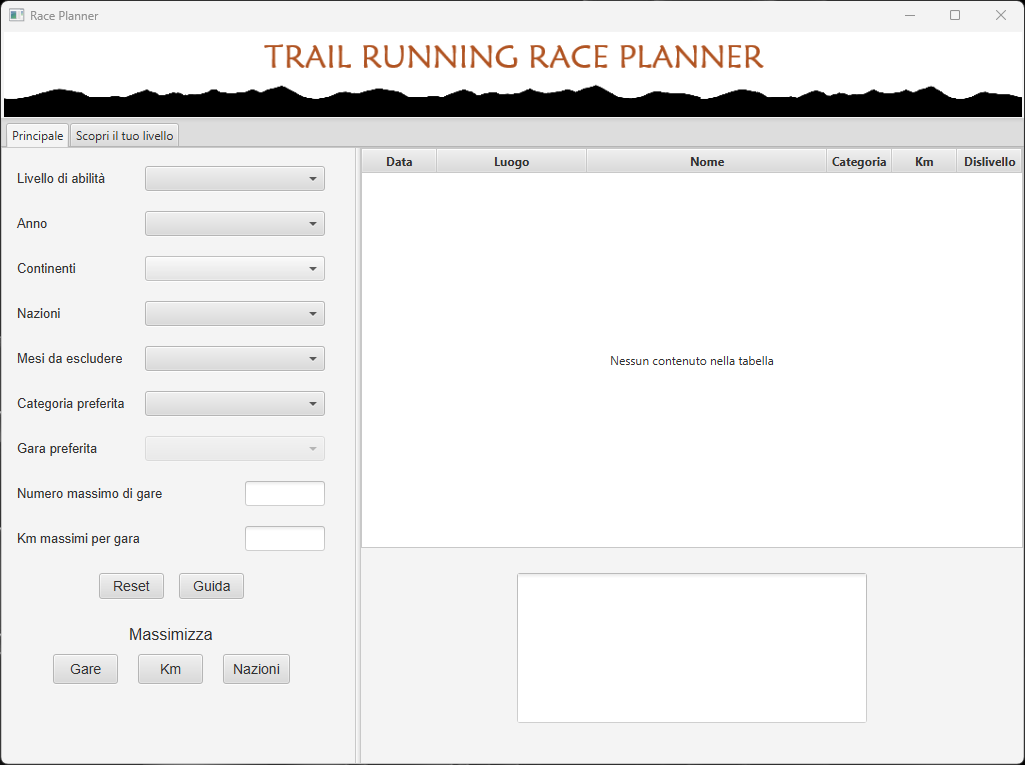
\includegraphics[width=0.9\textwidth]{images/tab_principale.png}
    \caption{Scheda Principale}
    \label{fig:tab-principale}
\end{figure}
% figura tab con risultato
\begin{figure}
    \centering
    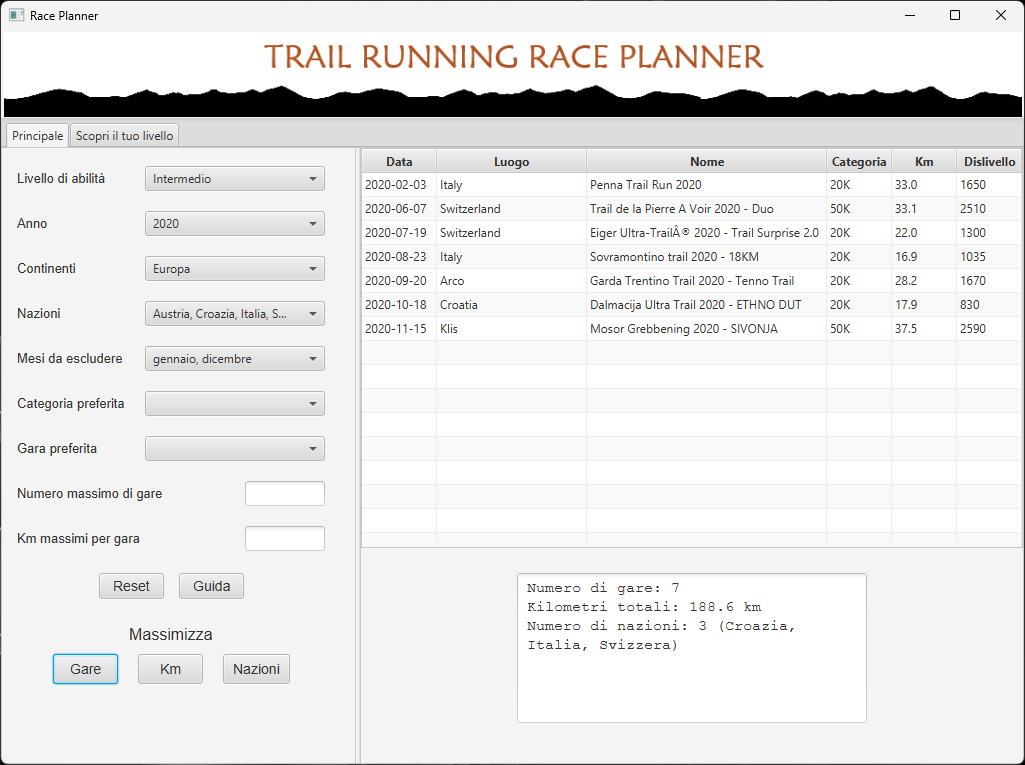
\includegraphics[width=0.9\textwidth]{images/tab_principale_soluzione.png}
    \caption{Scheda Principale con soluzione}
    \label{fig:tab-principale-soluzione}
\end{figure}
\newpage
Alla pressione del bottone \textit{Guida} è possibile visualizzare una seconda scena, mostrata come popup, contenente una breve guida per l'uso corretto dell'applicazione.
% figura con guida 
\begin{figure}[H]
    \centering
    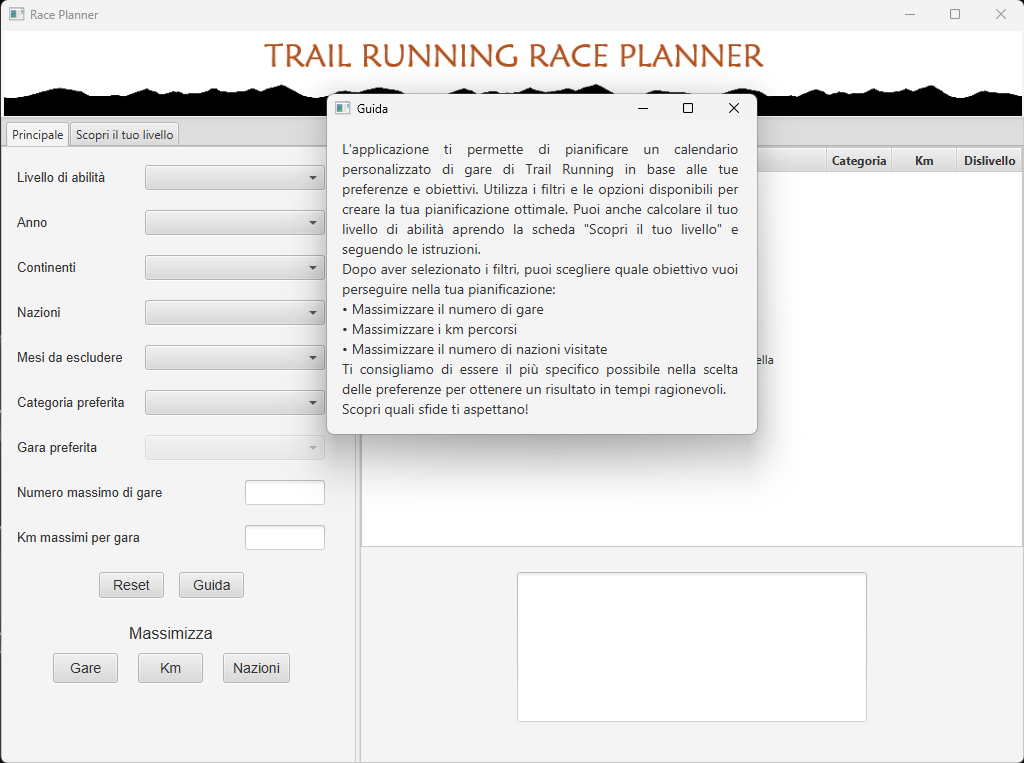
\includegraphics[width=0.9\textwidth]{images/scena_guida.png}
    \caption{Scena con guida}
    \label{fig:scena-guida}
\end{figure}
\newpage
La scheda \textit{Scopri il tuo livello} è costituita da vari campi di input, che l'utente può compilare con i dati opportuni, e da pulsanti. Alla pressione dell'apposito pulsante viene visualizzato il livello di abilità dell'utente, calcolato sulla base dei dati da lui/lei inseriti.
% figura con risultato
\begin{figure}[h]
    \centering
    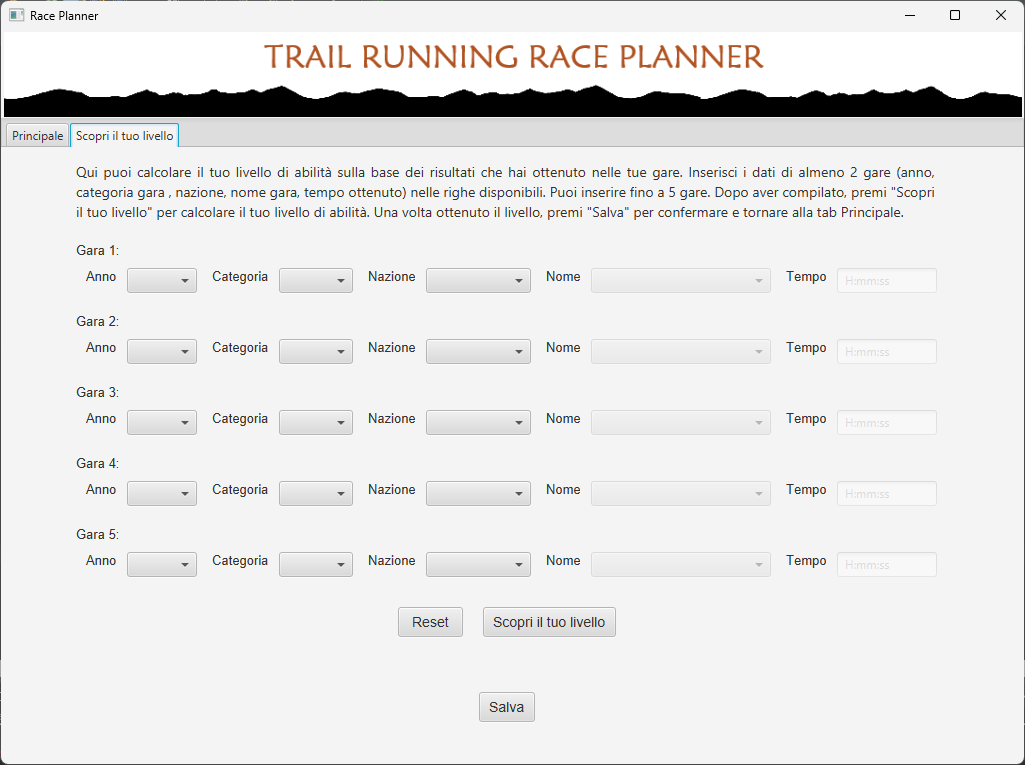
\includegraphics[width=0.9\textwidth]{images/tab_livello.png}
    \caption{Scheda Scopri il tuo livello}
    \label{fig:tab-livello}
\end{figure}

% link youtube 
Un video dimostrativo sull'uso dell'applicazione è disponibile al seguente link: {\color{blue}\url{https://youtu.be/I502-RbnuNU}}.

\chapter{Risultati sperimentali ottenuti}
Per ottenere la pianificazione delle gare, l'utente può impostare le proprie preferenze tramite i filtri disponibili e selezionare l'obiettivo desiderato premendo l'apposito pulsante.
Ad esempio, impostando il livello \textit{Intermedio}, l'anno \textit{2022}, le nazioni \textit{Repubblica Ceca, Romania, Slovacchia e Slovenia}, e i mesi da \textit{febbraio} a \textit{ottobre}, si ottengono le seguenti soluzioni:
% soluzione per gare
\begin{figure}[h]
    \centering
    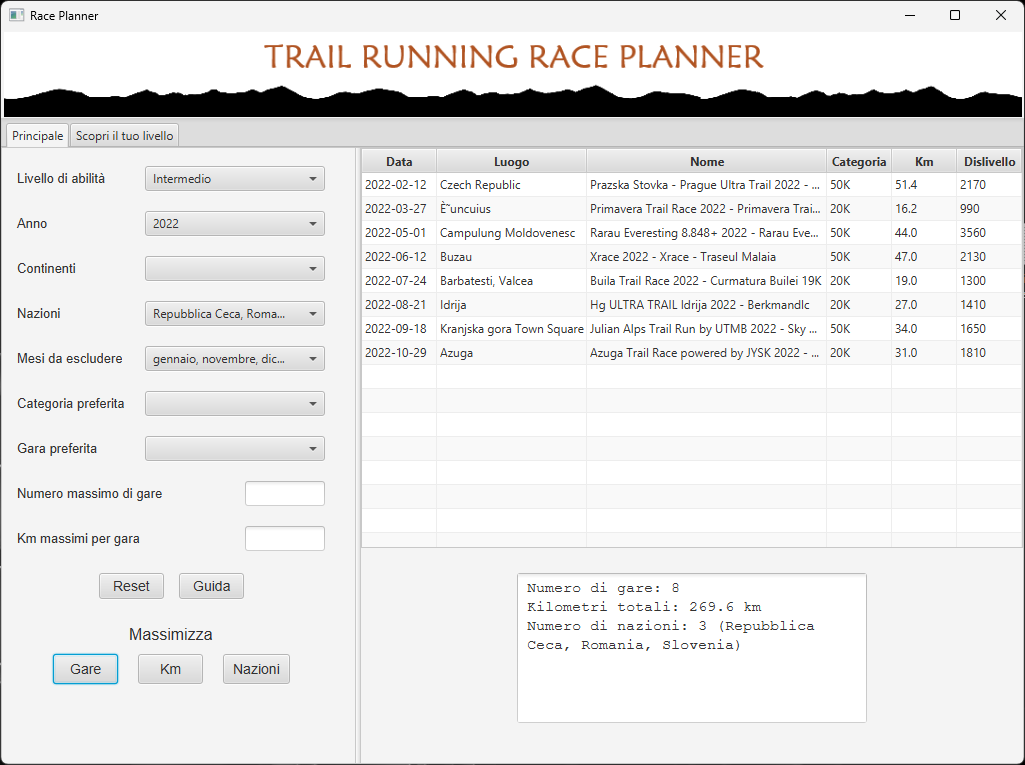
\includegraphics[width=0.8\textwidth]{images/esempio_gare.png}
    \caption{Esempio di Massimizza Gare}
    \label{fig:max-gare}
\end{figure}
% soluzione per km
\begin{figure}
    \centering
    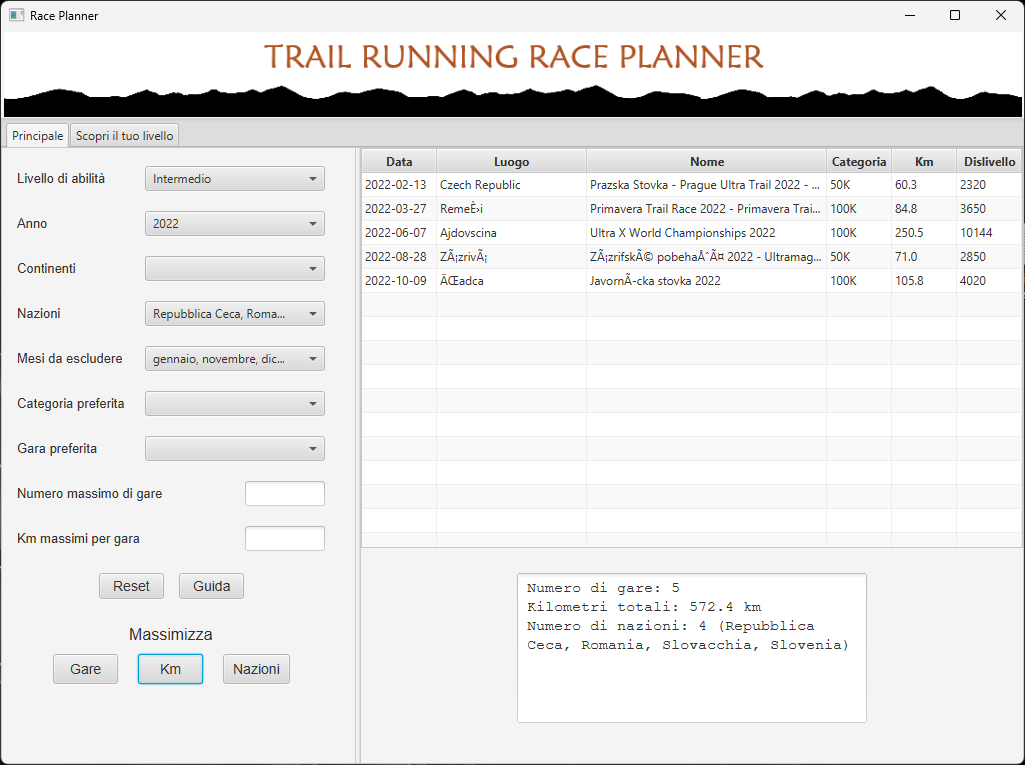
\includegraphics[width=0.8\textwidth]{images/esempio_km.png}
    \caption{Esempio di Massimizza Km}
    \label{fig:max-km}
\end{figure}
% soluzione per nazioni
\begin{figure}
    \centering
    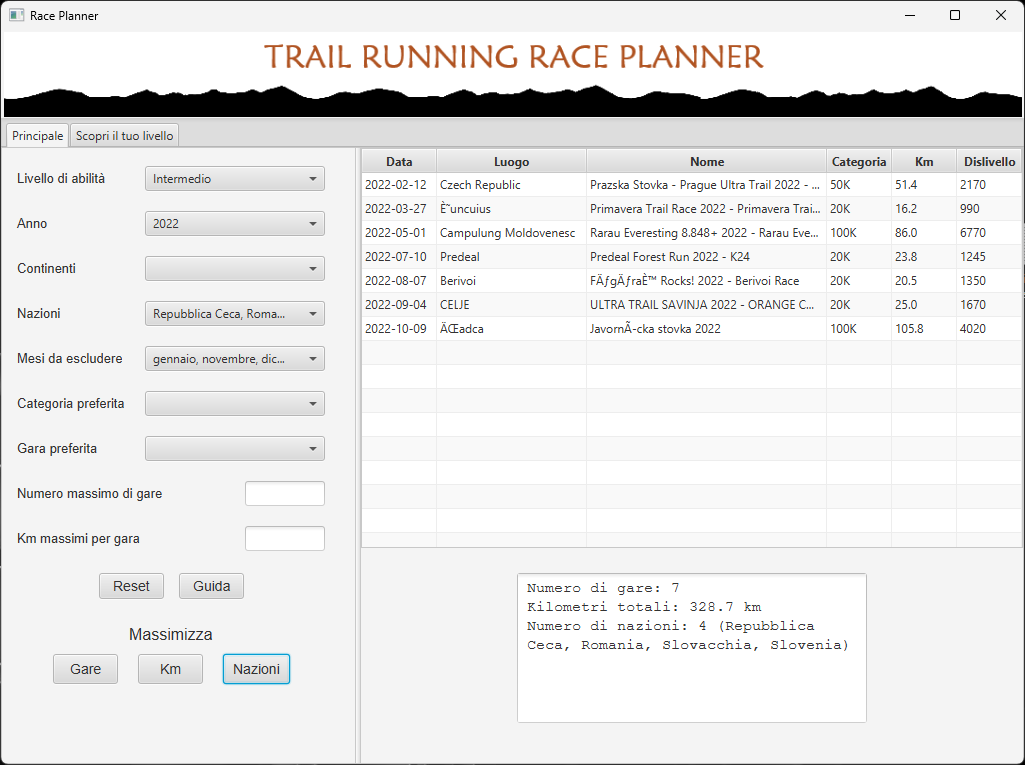
\includegraphics[width=0.8\textwidth]{images/esempio_nazioni.png}
    \caption{Esempio di Massimizza Nazioni}
    \label{fig:max-nazioni}
\end{figure}
\newpage
Come illustrato nelle immagini, gli obiettivi sono rispettatati: la soluzione in figura \ref{fig:max-gare} contiene il maggior numero di gare, i chilometri totali nella soluzione in figura \ref{fig:max-km} sono il valore più alto tra le tre soluzioni, e nella soluzione in figura \ref{fig:max-nazioni} sono incluse, in questo caso, tutte le nazioni selezionate.  

La scelta di una gara preferita, tramite l'apposito filtro, implica che tale gara farà sicuramente parte della soluzione. Viene mostrato un esempio:
\begin{figure}[h]
    \centering
    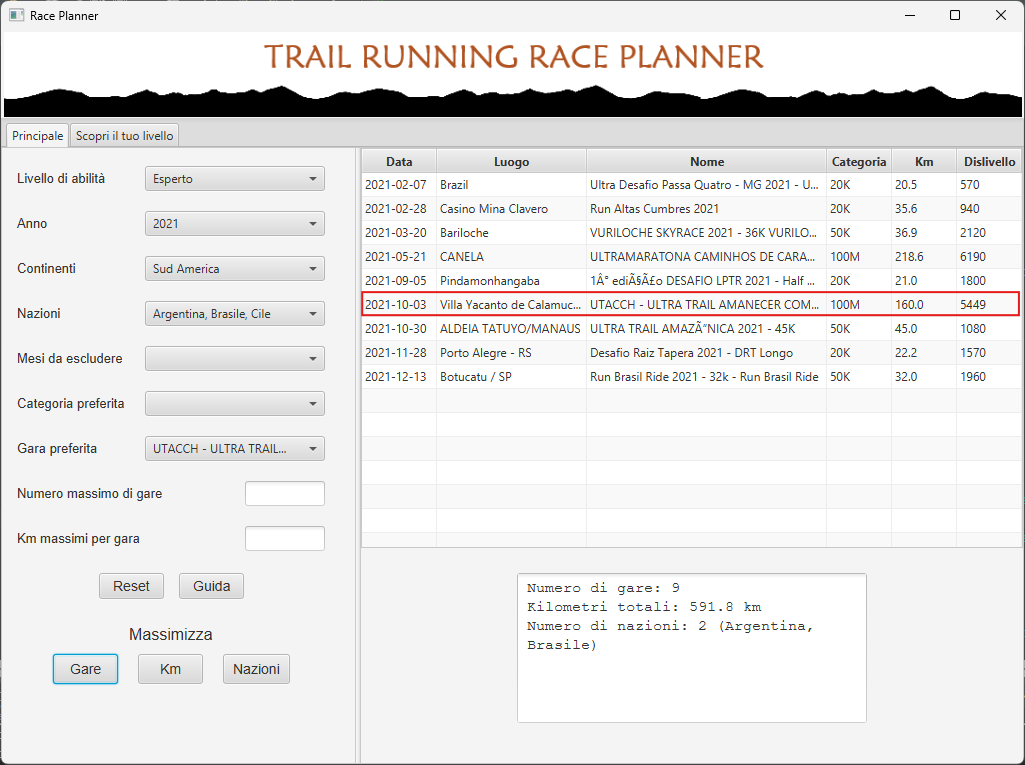
\includegraphics[width=0.8\textwidth]{images/esempio_favRace.png}
    \caption{Esempio gara preferita}
    \label{fig:gara-preferita}
\end{figure}
\newpage
Nella scheda \textit{Scopri il tuo livello}, l'utente può inserire i dati relativi ai risultati ottenuti nelle gare da lui/lei disputate. È necessario compilare i campi per almeno 2 gare per poter determinare il proprio livello di abilità. 
\begin{figure}[h]
    \centering
    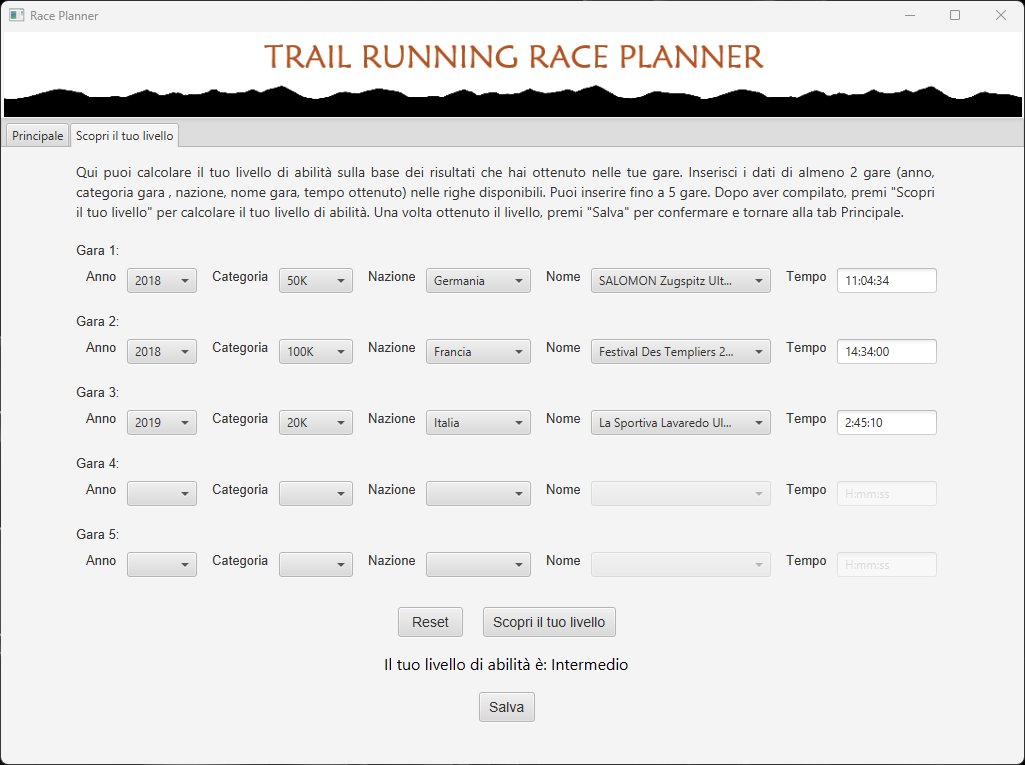
\includegraphics[width=0.8\textwidth]{images/esempio_livello.png}
    \caption{Esempio Scopri il tuo livello}
    \label{fig:es-livello}
\end{figure}

Ad ogni pulsante premuto è associato un determinato evento, gestito dal Controller. Tutti gli eventi prevedono controlli di validità sui dati inseriti; in presenza di errori, l'applicazione mostra all'utente le indicazioni su come correggerli.
\begin{figure}[h]
    \centering
    
\includegraphics[width=\textwidth]{images/esempio_errori.png}
    \caption{Esempio errori}
    \label{fig:es-errori}
\end{figure}

\chapter{Valutazioni sui risultati ottenuti e conclusioni}
L'applicazione sviluppata si dimostra uno strumento valido per il contesto operativo considerato. Gli obiettivi prefissati in fase di progettazione, descritti nel capitolo \ref{cap:proposta}, vengono raggiunti, nonostante i limiti prestazionali dell'algoritmo ricorsivo discussi nella sezione \ref{sec:algoritmi}. 

Per ridurre la complessità dell'algoritmo, si potrebbe adottare un approccio euristico, puntando ad una soluzione approssimata piuttosto che ottimale. Questa scelta risulterebbe più efficiente dal punto di vista computazionale, ma richiederebbe di riformulare gli obiettivi dell'applicazione. Sarebbe infatti necessario stabilire un livello di approssimazione accettabile per considerare valida una combinazione di gare, ma anche definire parametri concreti su cui basare tale approssimazione. Tuttavia, introdurre questi parametri potrebbe compromettere la realisticità dell'applicazione rispetto agli obiettivi per cui è stata progettata, dato che la natura stessa dell'approssimazione implica l'assenza di un criterio unico e preciso. I parametri definiti risulterebbero pertanto arbitrari, distaccandosi dal contesto realistico dell'applicazione.  

Per quanto riguarda l'esperienza d'uso, l'applicazione presenta un'interfaccia semplice e intuitiva, come illustrato nel capitolo \ref{cap:interfaccia}, offrendo all'utente uno strumento immediato e di facile utilizzo.

Questa applicazione potrebbe costituire la base per la realizzazione di una piattaforma completa dedicata al trail running, con l'aggiunta di nuove funzionalità: 
\begin{itemize}
    \item \textbf{Storico dell'atleta}: salvataggio dei risultati delle gare disputate, consentendo all'atleta di monitorare i propri progressi
    \item \textbf{Gestione di sorteggi e qualifiche}: monitoraggio dei metodi di iscrizione alle gare e verifica dei requisiti di accesso 
    \item \textbf{Piani di allenamento}: sviluppo di un piano di allenamento personalizzato per la preparazione alle gare
    \item \textbf{Sincronizzazione con dispositivi activity tracker}: acquisizione dei dati di performance dai dispositivi indossabili
    \item \textbf{Simulazione risultati}: stima dei risultati nelle gare in programma, basata sui dati raccolti dagli allenamenti e sullo stato di forma corrente
    \item \textbf{Sistema di notifiche}: invio di promemoria per scadenze delle iscrizioni
\end{itemize}
Chiaramente, una piattaforma di questo tipo deve essere supportata da dataset estremamente dettagliati e costantemente aggiornati. Inoltre, la sua implementazione richiederebbe una gestione complessa e un'infrastruttura robusta. Tuttavia, questo investimento potrebbe tradursi in uno strumento completo e potenzialmente competitivo nel mercato del trail running.

In conclusione, l'applicazione sviluppata si rivela un'efficace risorsa per atleti e appassionati di trail running, facilitando l'organizzazione delle loro attività sportive. 

\newpage
\section*{Licenza d'uso}
\doclicenseThis
\end{document}